%% See: https://bookdown.org/yihui/rmarkdown-cookbook/multi-column.html
%% I've made some additional adjustments based on my own preferences (e.g. cols
%% should be top-aligned in case of uneven vertical length)
\newenvironment{columns}[1][]{}{}

\newenvironment{column}[1]{\begin{minipage}[t]{#1}\ignorespaces}{%
\end{minipage}
\ifhmode\unskip\fi
\aftergroup\useignorespacesandallpars
}

\def\useignorespacesandallpars#1\ignorespaces\fi{%
#1\fi\ignorespacesandallpars}

\makeatletter
\def\ignorespacesandallpars{%
  \@ifnextchar\par
    {\expandafter\ignorespacesandallpars\@gobble}%
    {}%
}
\makeatother


\title [Nonparametrics]{Nonparametrics and Local Methods: Kernels}
\author{C.Conlon}
\institute{Applied Econometrics}
\date{\today}
\setbeamerfont{equation}{size=\tiny}
\begin{document}

\begin{frame}
\titlepage
\end{frame}


\begin{frame}{Big Data}
\begin{itemize}
\item It used to be that if you had $N=50$ observations then you had a lot of data.
\item Those were the days of finite-sample adjusted t-statistics.
\item Now we frequently have 1 million observations or more, why can't we use k-NN type methods everywhere?
\end{itemize}
\end{frame}

\begin{frame}{Curse of Dimensionality}
Take a unit hypercube in dimension $p$ and we put another hypercube within it that captures a fraction of the observations $r$ within the cube
\begin{itemize}
\item Since it corresponds to a fraction of the unit volume, $r$ each edge  will be $e_p(r) = r^{1/p}$.
\item $e_{10}(0.01) = 0.63$ and $e_{10}(0.1) = 0.80$, so we need almost 80\% of the data to cover 10\% of the sample!
\item If we choose a smaller $r$ (include less in our average) we increase variance quite a bit without really reducing the required interval length substantially.
\end{itemize}
\end{frame}

\begin{frame}{Curse of Dimensionality}
\begin{figure}[htbp]
\begin{center}
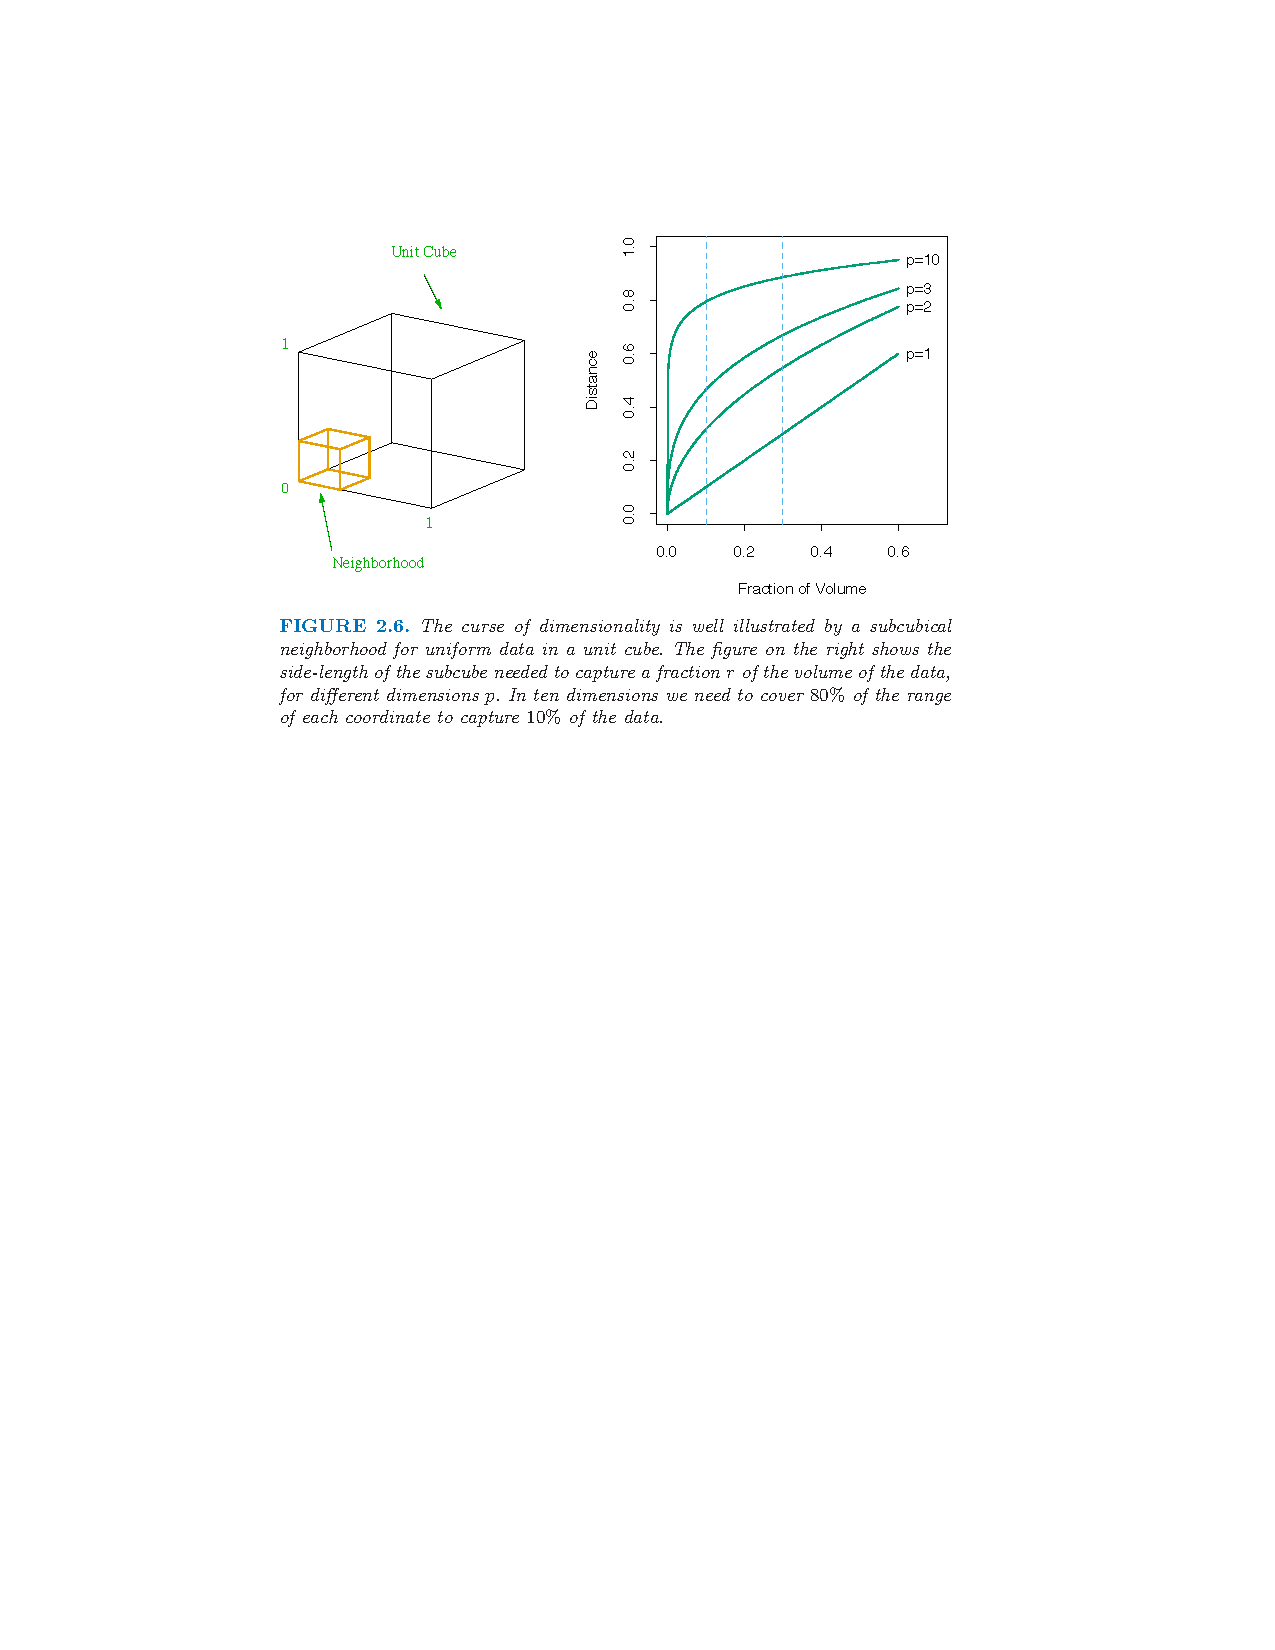
\includegraphics[width=3.5in]{./resources/figure26.pdf}
\label{class15nn}
\end{center}
\end{figure}
\end{frame}

\begin{frame}{Curse of Dimensionality}
Don't worry, it only gets worse:
\begin{eqnarray*}
d(p,N) = \left(1-\left(\frac{1}{2} \right)^{1/N} \right)^{1/p}
\end{eqnarray*}

\begin{itemize}
\item $d(p,N)$ is the distance from the origin to the closest point.
\item $N=500$ and $p=10$ means $d = 0.52$ or that the closest point is closer to the boundary than the origin!
\item Why is this a problem?
\item In some dimension nearly every point is the closest point to the boundary -- when we average over nearest neighbors we are \alert{extrapolating} not \alert{interpolating}.
\end{itemize}
\end{frame}


\begin{frame}{Density/Distribution Estimation}
One of the more successful and popular uses of nonparametric methods is estimating the density or distribution function $f(x)$ or $F(x)$.
\begin{itemize}
\item Estimating the CDF is easy and something you have already done
\item Q-Q plots, etc.
\end{itemize}
\begin{eqnarray*}
\hat{F}_{ECDF}(x_0) = \frac{1}{N} \sum_{i=1}^N (x_i \leq x_0 )
\end{eqnarray*}
\begin{itemize}
\item Differentiating to get density is unhelpful : $F_{ECDF}'(x) = 0$ in most places.
\end{itemize}
\end{frame}

\begin{frame}{Density/Distribution Estimation}
One of the more successful and popular uses of nonparametric methods is estimating the density or distribution function $f(x)$ or $F(x)$.
\begin{itemize}
\item Think about the histogram (definition of derivative):
\begin{eqnarray*}
\hat{f}_{HIST}(x_0) = \frac{1}{N} \sum_{i=1}^N \frac{\mathbf{1}(x_0 - h < x_i < x_0 + h)}{2 h}
\end{eqnarray*}
\end{itemize}
\end{frame}

\begin{frame}{Density/Distribution Estimation}
\begin{itemize}
\item Divide the dataset into bins, count up fraction of observations in each bins
\item Similar to k-NN except instead of windows that vary with $x_i$ we have fixed width bins
\item Larger bin width $\rightarrow$ More Bias, Less Variance.
\item Histogram will never be smooth! (Just like k-NN).
\end{itemize}
\begin{eqnarray*}
\hat{f}_{HIST}(x_0) = \frac{1}{Nh} \sum_{i=1}^N  \frac{1}{2} \cdot \mathbf{1} \left (\left|\frac{x_i - x_0}{h} \right| < 1 \right)
\end{eqnarray*}
\end{frame}




\begin{frame}{Smooth Kernels}
We can take our histogram and smooth it out:
\begin{eqnarray*}
\hat{f}(x_0) = \frac{1}{Nh} \sum_{i=1}^N  K  \left(\frac{x_i - x_0}{h} \right)  \frac{1}{n}\sum_{i=1}^n K_h\left(
y-y_i\right).
\end{eqnarray*}
We call $K(\cdot)$ a \alert{Kernel function} and $h$ the \alert{bandwidth}. We usually assume
\begin{enumerate}[(i)]
\item $K(z)$ is symmetric about $0$ and continuous.
\item $\int K(z) d z = 1$,  $\int z K(z) d z = 0$,  $\int |K(z)| d z < \infty$.
\item Either (a) $K(z) = 0$ if $|z| \geq z_0$ for some $z_0$ or \\
(b) $|z| K(z) \rightarrow 0$ as $|z| \rightarrow \infty$.
\item $\int z^ K(z) d z = \kappa$ where $\kappa$ is a constant.
\end{enumerate}
\end{frame}

\begin{frame}{Kernel Smoothers}
If $K$ is $C^k$, then so is ${\hat f}_n$, so we can plot it nicely.

\pause

Usually we choose a smooth, symmetric $K$:



\pause




\begin{itemize}[<+->]
\item $K=\phi$, density of $N(0,1)$ (or some other symmetric density);
\item $K$ with compact support: Epanechnikov (mildly) optimal
\[
K(x)= \frac{3}{4} \max(1-x^2,0).
\]
\end{itemize}
\pause
A common nonsmooth choice: $K(x)=(|x|<1/2)$ gives the {\em histogram}
estimate.
\end{frame}

\begin{frame}{Kernel Comparison}
\begin{figure}[htbp]
\begin{center}
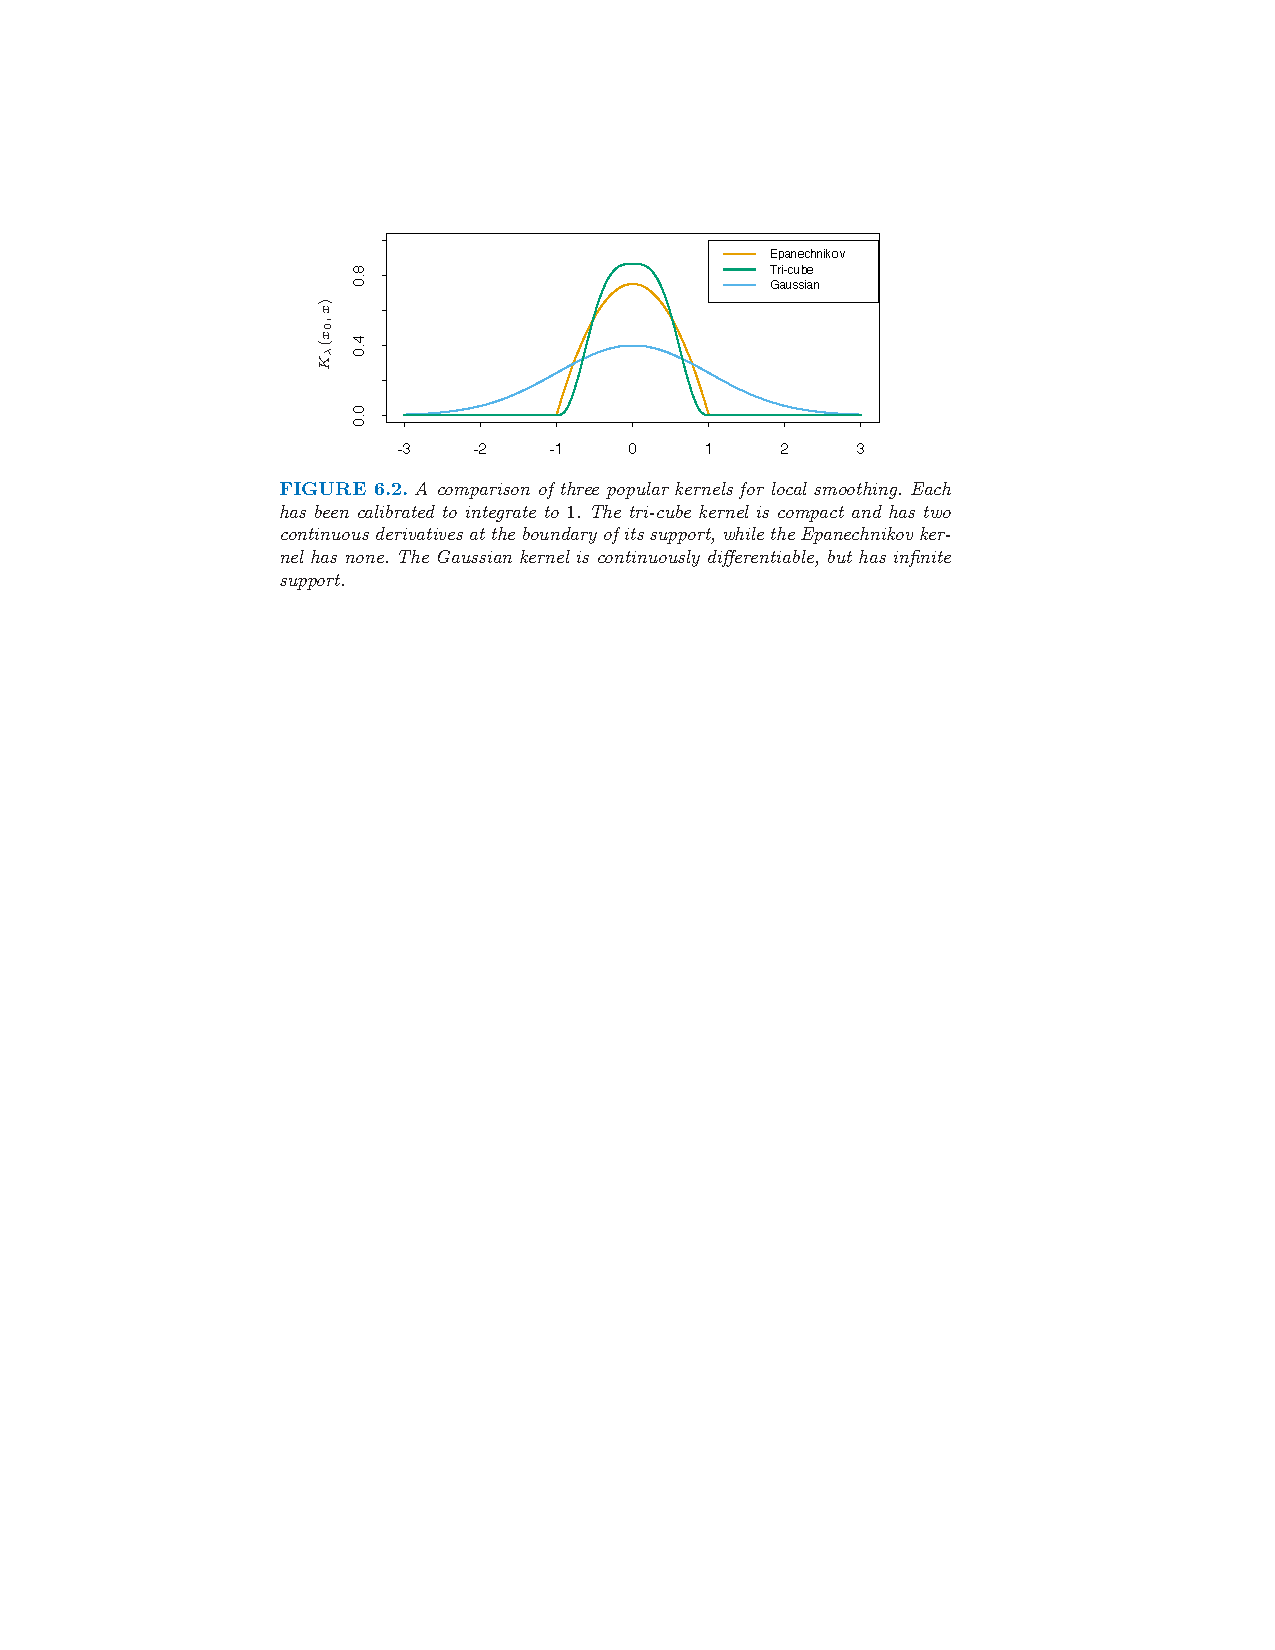
\includegraphics[width=3.5in]{./resources/kernelfig.pdf}
\label{classOLS}
\end{center}
\end{figure}
\end{frame}


\begin{frame}{How to Choose $h$}
\begin{itemize}
\item We want both bias and variance to be as small as possible, as usual. 
\item In parametric estimation, it is not a problem: they both go to zero as sample size increases.
\end{itemize}
 {\bf Problem with nonparametrics:}
$$E\hat{f}_n(y)=\int K((y-t)/h)f(t)dt/h=\int K(-u)f(y+uh)du=f(y)+O(h^2)$$
$\rightarrow$ bias can be made tiny by having a very concentrated kernel ($h\simeq 0$);
but 
$$V\hat{f}_n(y)=\frac{1}{nh^2}VK((y-Y)/h)=O\left(\frac{1}{nh}\right)$$
$\rightarrow$ a small $h$ gives a high variance! \\
Reducing $h$ reduces bias, but increases variance; how are we to
trade off?
\end{frame}

\begin{frame}{The AMISE}
\begin{itemize}
\item  Asymptotic Mean Integrated Square Error =asymptotic approximation of a quadratic loss function
$$E\left({\hat f}_n(y)-f(y)\right)^2 dy$$
\item Simple approximate expression (symmetric kernels of order 2): $$(\mbox{bias})^2+\mbox{variance}= A
h^4+B/nh$$
\item {\bf Why?} Bias in $y$ is
$$
\int K(-u)\left(f(y+uh)-f(y)\right)du \simeq h^2 \frac{f''(y)}{2}\int K(u)u^2 du.
$$
{\em Intuition:} if $f$ is close to linear around $y$, then averaging
does not hurt us: $f"(y)\simeq 0$ and the bias is small. The bias is larger  (and negative) at the mode of $f$.
\end{itemize}
\end{frame}

\frame{\frametitle{The Variance}

\pause

\[
V\hat{f}_n(y)=\frac{1}{nh^2} VK((y-Y)/h)
\]

\pause

The important term in 
\[
VK((y-Y)/h)
\]
is 
\[
h\int K(u)^2 f(y+uh)du\simeq h f(y)\int K(u)^2 du.
\]

\pause

And we end up with 
\[
V\hat{f}_n(y) \simeq \frac{f(y)}{nh} \int K(u)^2du.
\]

\pause

{\em Intuition:} we are really taking an average over $nhf(y)$
points. In low-density region, this induces a high \emph{relative\/}
imprecision:
\[
\frac{\sigma(\hat{f}_n(y))}{f(y)}=\frac{1}{nhf(y)} \int K(u)^2du.
\]
 }

\frame{\frametitle{Optimal bandwidth}
\begin{itemize}
\item The AMISE is $$Ah^4+B/nh$$
 with $A=\int \left(f''(y)\right)^2 \left(\int u^2K\right)^2 /4$ and $B=f(y)\int K^2$
\item  AMISE is
smallest in $h^*_n=\left(\frac{B}{4An}\right)^{1/5}$. Then,
\begin{itemize}[<+->]
\item bias and standard error are \emph{both} in $n^{-2/5}$
\item and the AMISE is $n^{-4/5}$---{\bf not} $1/n$ as it is in parametric models.
\end{itemize}
\item But: $A$ and $B$ both depend on $K$ (known) and $f(y)$ (unknown), and
especially ``wiggliness''
$\int (f'')^2$ (unknown, not easily estimated). Where do we go from here? 
\end{itemize}
}


\frame{\frametitle{Silverman's Rule of Thumb}
\begin{itemize}
\item If $f$ is normal with variance $\sigma^2$ (may not be a very appropriate benchmark!), the optimal bandwidth
is
$$h^*_n=1.06 \sigma n^{-1/5}$$
\item Just do it with $\sigma=s$ empirical dispersion of the $y_i$'s , or
something more robust/slightly less smooth:
$$h^*_n=0.9*\min(s,IQ/1.34)*n^{-1/5}, \; \mbox{IQ=interquartile
 distance}$$
\item Investigate changing it by a reasonable multiple.
\end{itemize}
}


\end{document}